\documentclass[onecolumn, draftclsnofoot,10pt, compsoc]{IEEEtran}
\usepackage{graphicx}
\usepackage{url}
\usepackage{setspace}
\usepackage{caption}
\usepackage{subcaption}
\graphicspath{ {Images/} }
\usepackage{geometry}
\usepackage{imakeidx}
\makeindex[columns=1, options=-s lou3.ist]
\geometry{textheight=9.5in, textwidth=7in}

% 1. Fill in these details
\def \CapstoneTeamName{   The Visionaries}
\def \CapstoneTeamNumber{   3}
\def \GroupMemberOne{     Kien Tran}
\def \GroupMemberTwo{       Brian Wiltse}
\def \CapstoneProjectName{    Code3 Visionary}
\def \CapstoneSponsorCompany{ Levrum Data Technologies}
\def \CapstoneSponsorPerson{  Carl Niedner}

% 2. Uncomment the appropriate line below so that the document type works
\def \DocType{    
        %Requirements Document
        % Review
        %Design Document
        Midterm Progress Report
        }
      
\newcommand{\NameSigPair}[1]{\par
\makebox[2.75in][r]{#1} \hfil   \makebox[3.25in]{\makebox[2.25in]{\hrulefill} \hfill    \makebox[.75in]{\hrulefill}}
\par\vspace{-12pt} \textit{\tiny\noindent
\makebox[2.75in]{} \hfil    \makebox[3.25in]{\makebox[2.25in][r]{Signature} \hfill  \makebox[.75in][r]{Date}}}}
\newcommand{\tabitem}{~~\llap{\textbullet}~~}
% 3. If the document is not to be signed, uncomment the RENEWcommand below
\renewcommand{\NameSigPair}[1]{#1}

%%%%%%%%%%%%%%%%%%%%%%%%%%%%%%%%%%%%%%%
\begin{document}

\begin{titlepage}
    \pagenumbering{gobble}
    \begin{singlespace}
      
\includegraphics[height=4cm]{coe_v_spot1}
        \hfill 
        % 4. If you have a logo, use this include graphics command to put it on the cover sheet.
        %\includegraphics[height=4cm]{CompanyLogo}   
        \par\vspace{.2in}
        \centering
        \scshape{
            \huge CS Capstone \DocType \par
            \large{Winter Term}\par
            {\large\today}\par
            \vspace{.5in}
            \textbf{\Huge\CapstoneProjectName}\par
            \vfill
            {\large Prepared for}\par
            \Huge \CapstoneSponsorCompany\par
            \vspace{5pt}
            {\Large\NameSigPair{\CapstoneSponsorPerson}\par}
            {\large Prepared by }\par
            Group\CapstoneTeamNumber\par
            % 5. comment out the line below this one if you do not wish to name your team
            \CapstoneTeamName\par 
            \vspace{5pt}
            {\Large
                \NameSigPair{\GroupMemberOne}\par
                \NameSigPair{\GroupMemberTwo}\par
            }
            \vspace{20pt}
        }
        \begin{abstract}
                Over the last ten weeks, our team has continued to work on Code3 Visionary, a project that aims to predict emergency services need in a given time and location. 
                We have made considerable progress in obtaining and consolidating the data required to perform statistical analyses for baseline measurements and to begin developing our machine learning module.
                This document summarizes our activities over Winter Break and the first five weeks of Winter Term.
        \end{abstract}
    \end{singlespace}
\end{titlepage}
\newpage
\pagenumbering{arabic}
\tableofcontents
% 7. uncomment this (if applicable). Consider adding a page break.
\listoffigures
%\listoftables
\clearpage

% 8. now you write!
\section{Introduction}
\begin{singlespace}
Our project, Code3 Visionary (C3V), is an application designed to predict how many emergency calls, and what types of emergency calls, will occur in a given time and place. 
C3V involves gathering data, researching and implementing machine learning algorithms, building an API, and building a minimal user interface that can display C3V's results. 
As we mentioned in our prior progress report, Code3 Visionary is a collaborative project with software engineers at Levrum, and our project specifications are subject to change depending on the needs of the Levrum team.
For the most part, our project focus has followed steps laid out in our Design Document;
however, we have been focusing more on a proof of concept for potential customers in Mecklenburg County, North Carolina, rather than a generalized application.

The remainder of this document summarizes what progress we made over Winter Break and in the first five weeks of Winter Term.
Section \ref{brian_weekly_summ} provides a description of Brian Wiltse's work on the project and what work is remaining.
Section \ref{kien_weekly_summ} provides a description of Kien Tran's work and what remains for him to complete.

\end{singlespace}

\section{Brian's Section} \label{brian_weekly_summ}
\begin{singlespace}
\subsection{Winter Break}
Over Winter Break, I began work on obtaining and transforming data required for emergency call predictions. I developed a Python program to convert a state shapefile from the United States Census into a county shapefile that contains demographics for each Census tract of the target county. Census tracts are subdivisions that make up a county. 

The Census provides shapefiles of states with basic geographic information (see Figure \ref{fig:nc_shp}).  However, our analyses and prediction algorithms will need a shapefile of an area that is a close approximation of a given emergency department's response area. Trimming the shapefile down to a target county and appending demographic information to each tract, which is a record within the shapefile, gives us the ability to have all information pertaining to each tract of a county in one location.

\begin{figure}[h!]
    \centering
    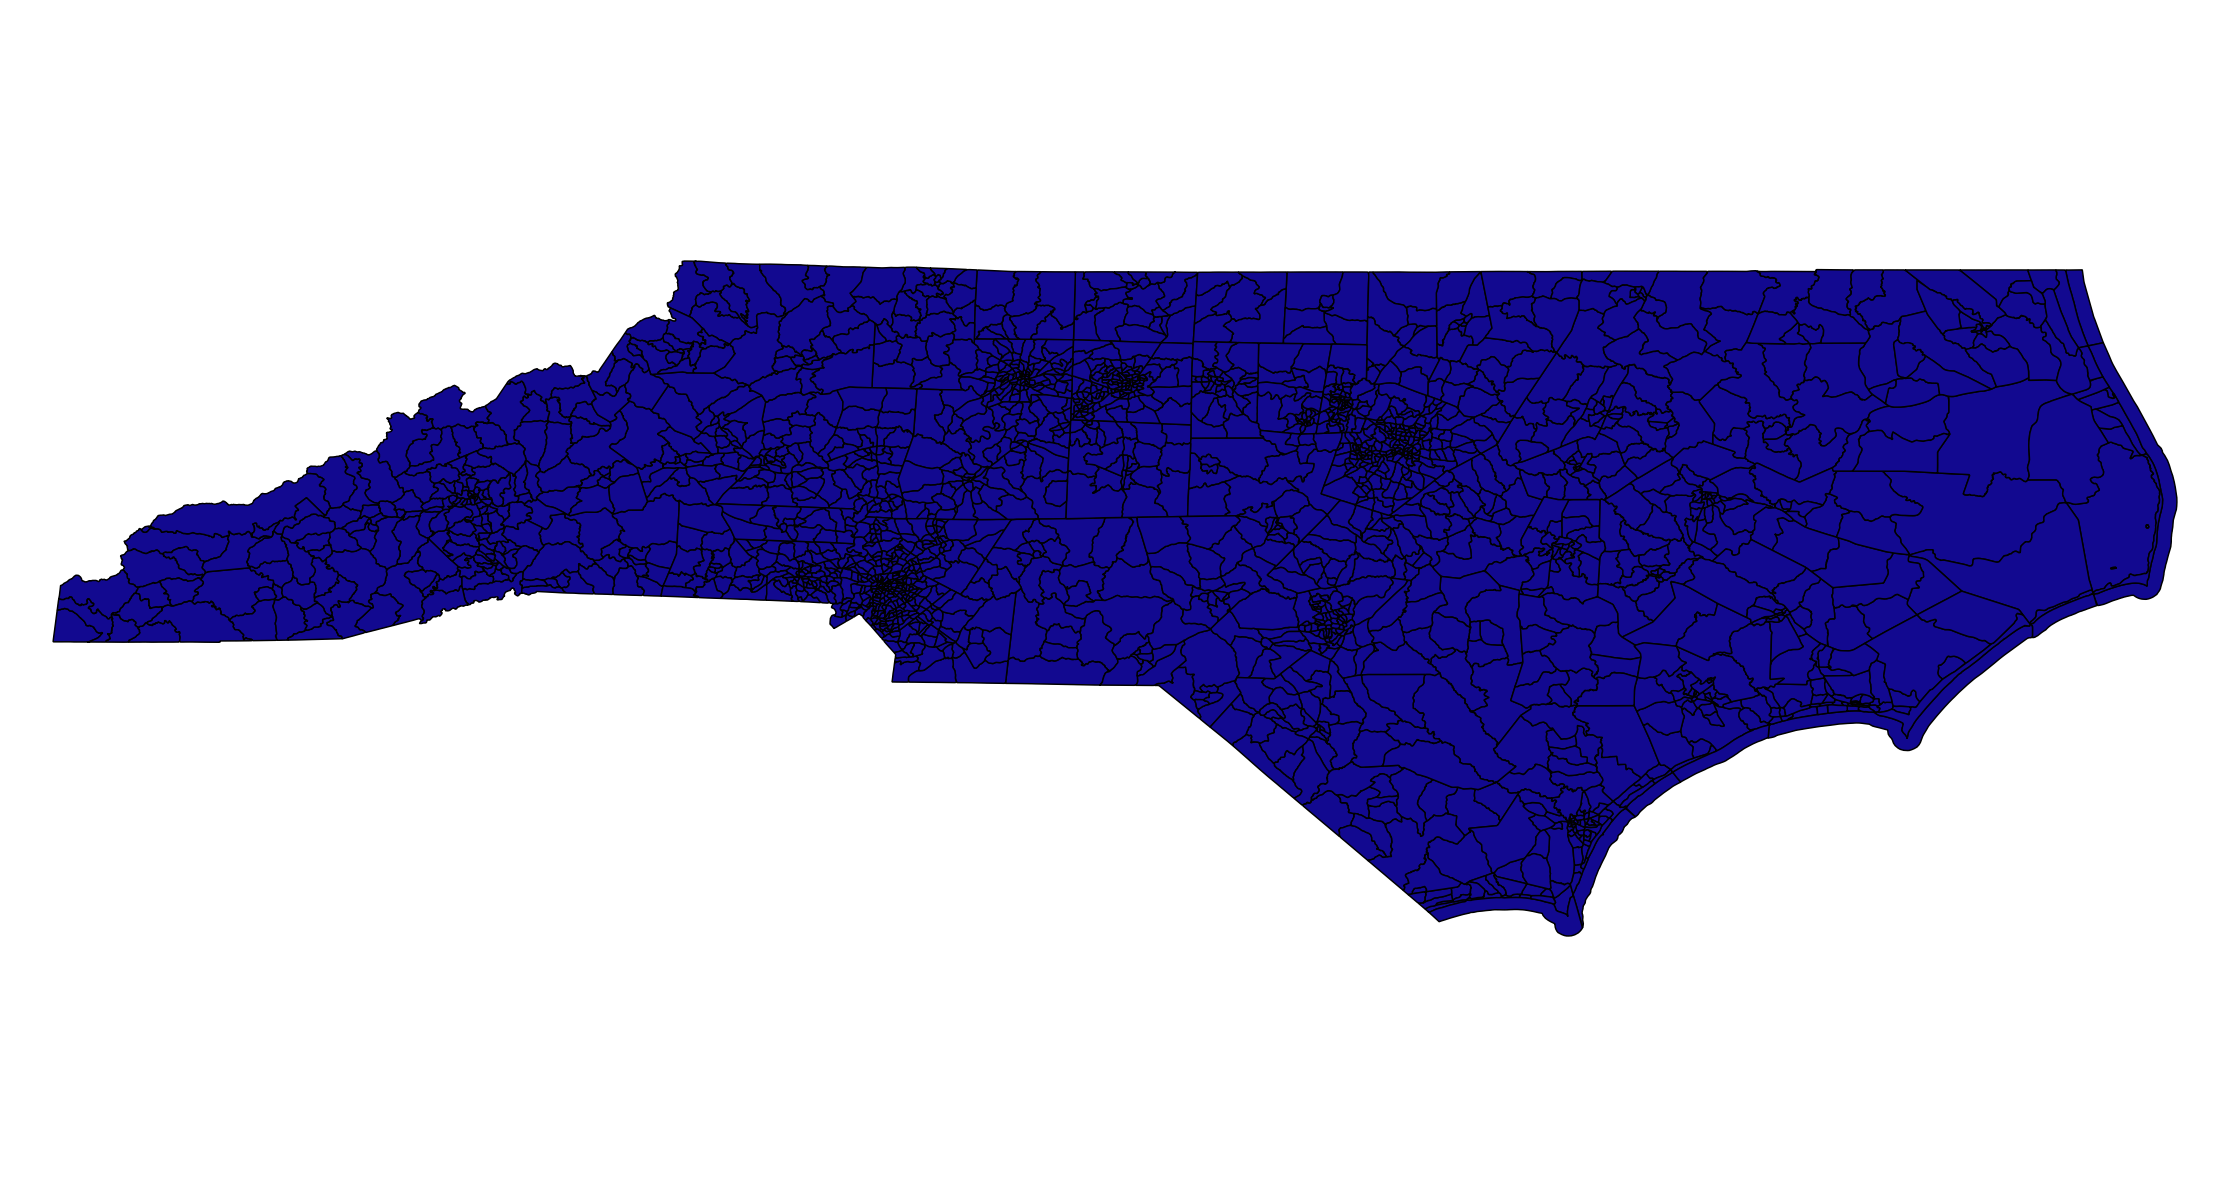
\includegraphics[scale=0.25]{NC.eps}
    \caption{Census Shapefile for North Carolina}
    \label{fig:nc_shp}
\end{figure}

The program creates a new shapefile in two main phases. First, it obtains all demographics for each Census tract of the target county. Then the program iterates through the records of the state shapefile, keeping only records from the target county and appending the demographic data to those records, which can be seen in the shapefile's attribute table (see Figure \ref{fig:att_tbl}). The retained records are then used to create the new shapefile (see Figure \ref{fig:nc_meck_shp}). In addition, I created a suite of unit tests and randomized tests that ensures the correct demographics are attributed to the correct tract.

\begin{figure}[h!]
    \centering
    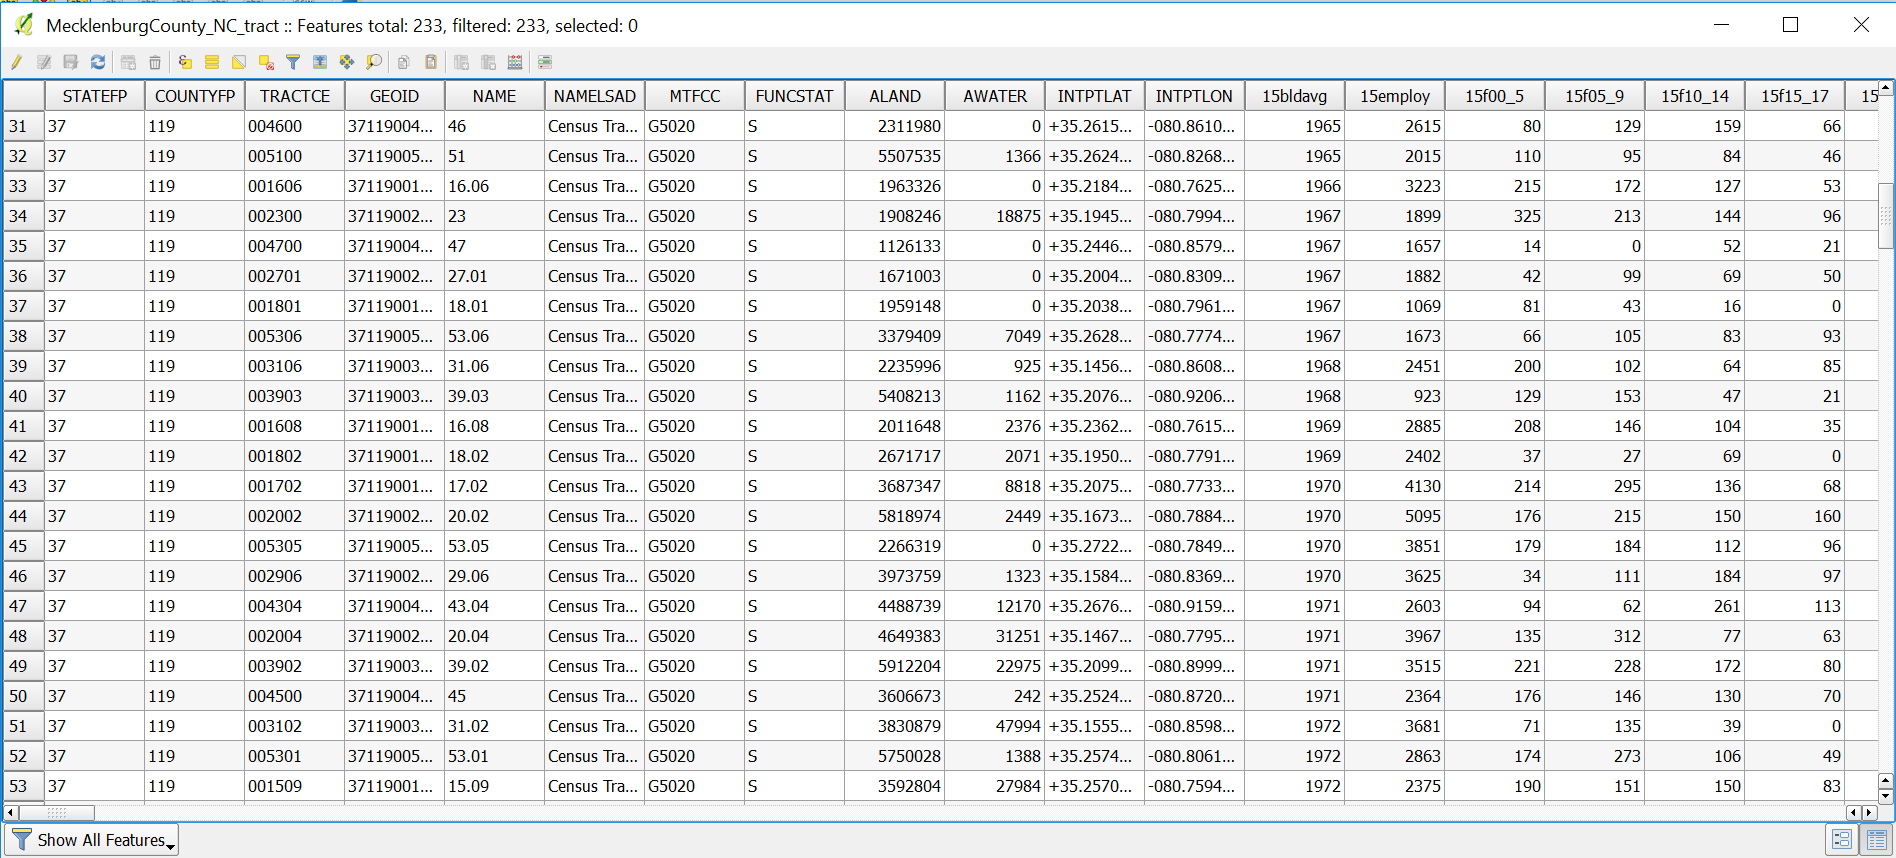
\includegraphics[scale=0.5]{att_tbl.eps}
    \caption{Mecklenburg County shapefile attribute table}
    \label{fig:att_tbl}
\end{figure}


\begin{figure}[h!]
    \centering
    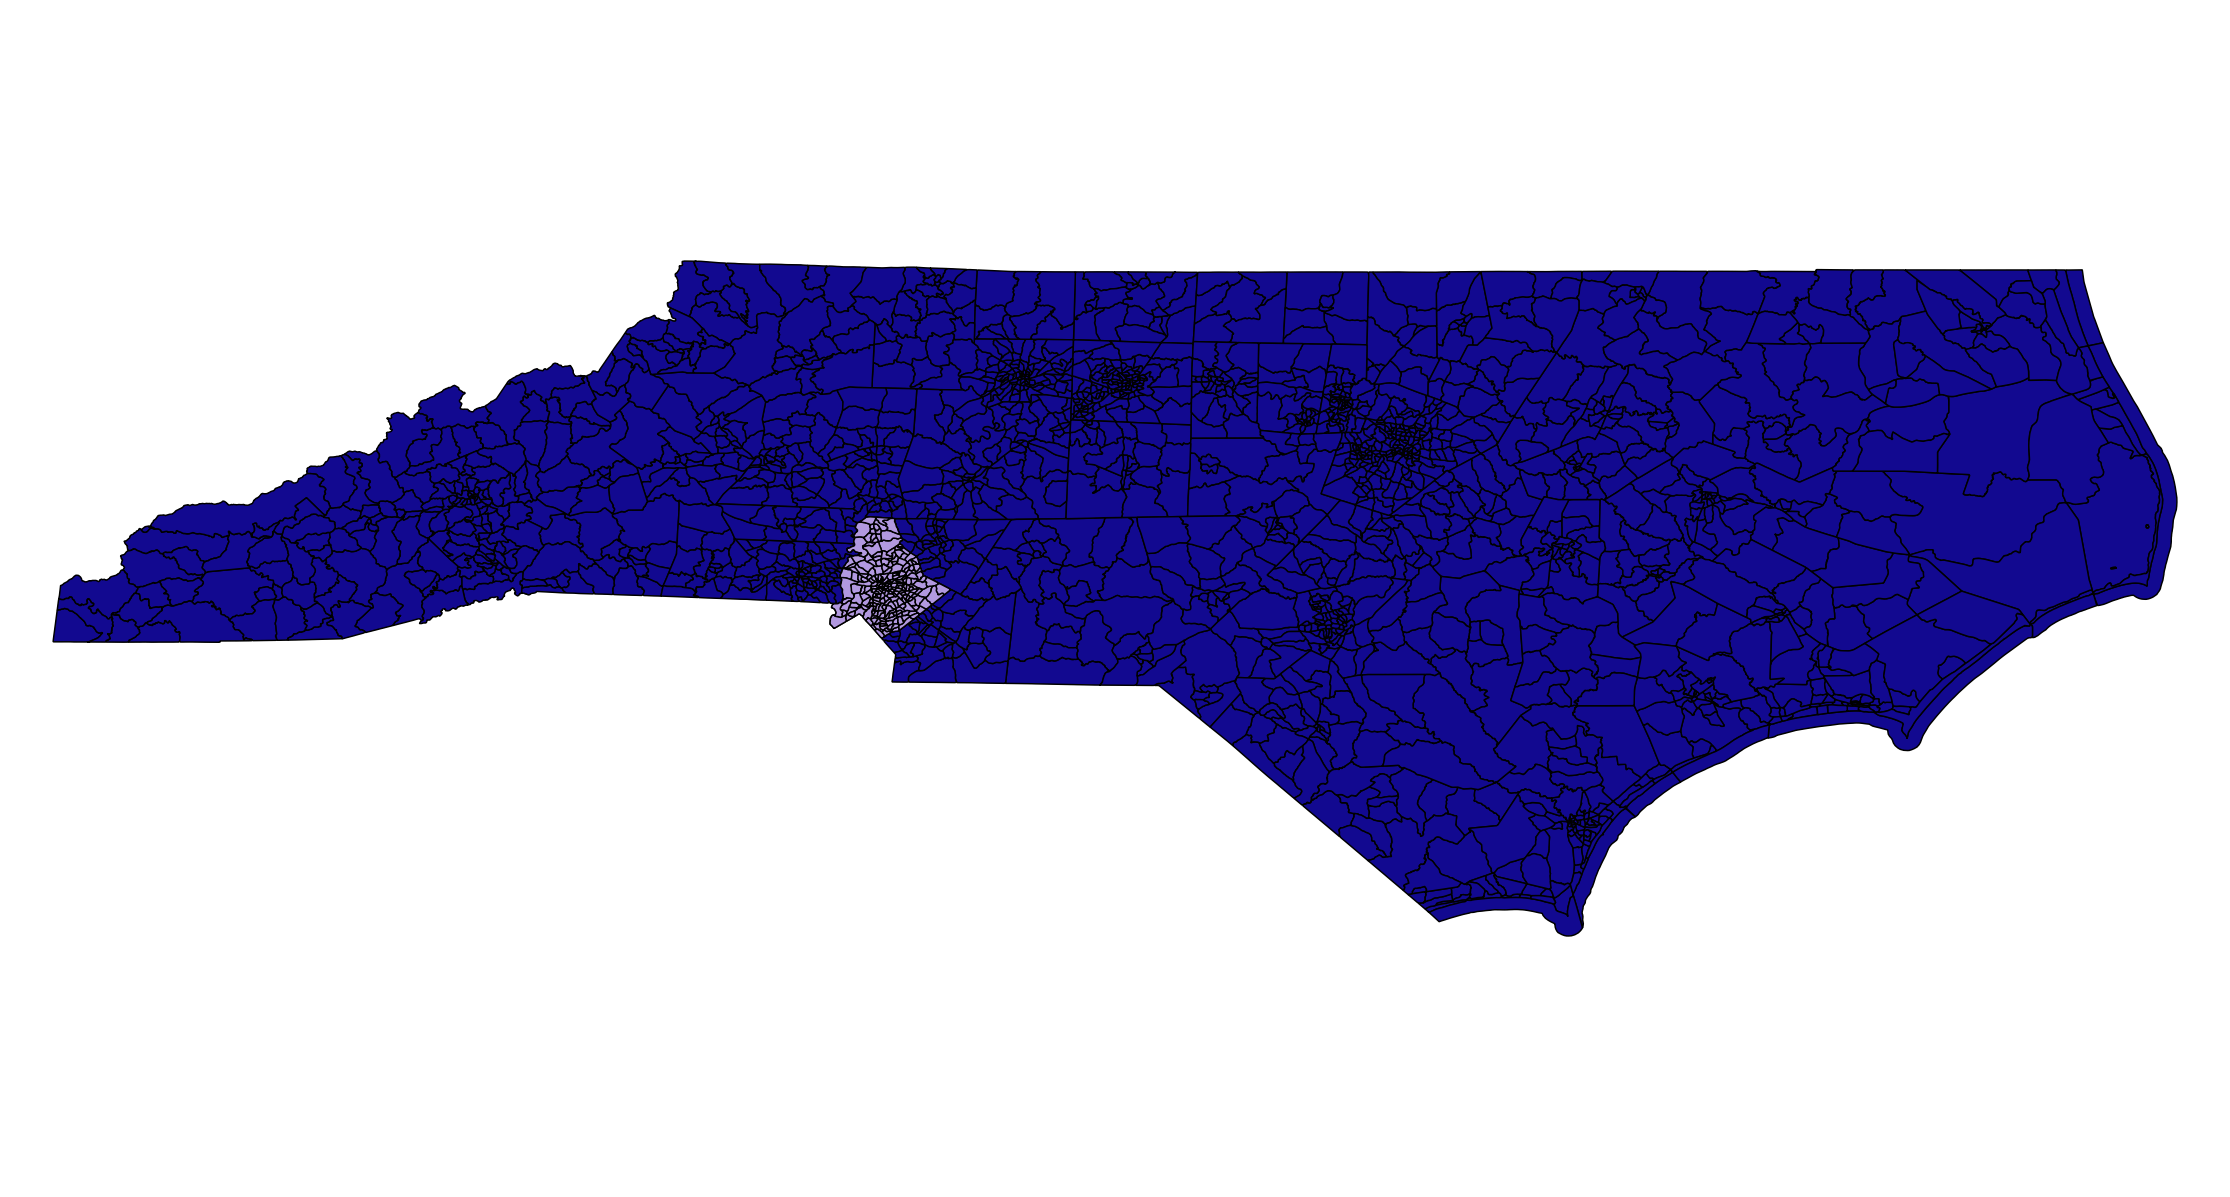
\includegraphics[scale=0.25]{NC_Meck.eps}
    \caption{Generated shapefile of Mecklenburg County (purple) overlaid on Census shapefile of North Carolina}
    \label{fig:nc_meck_shp}
\end{figure}

In addition to work on the shapefile conversion program, Kien and I had two remote meetings with Levrum to report on progress. The shapefile program worked specifically for Mecklenburg County, North Carolina at the time of the first meeting. By the second meeting, the program was generalized to work for all counties in the United States. During the second meeting, Carl further identified that we would need to get more granular information by obtaining data for each Census block group. A block group is a subdivision of a Census tract (see \ref{fig:meck_bg}). I worked on obtaining data for each block group over the remainder of the break.


\begin{figure}
\centering
\begin{subfigure}{.5\textwidth}
  \centering
  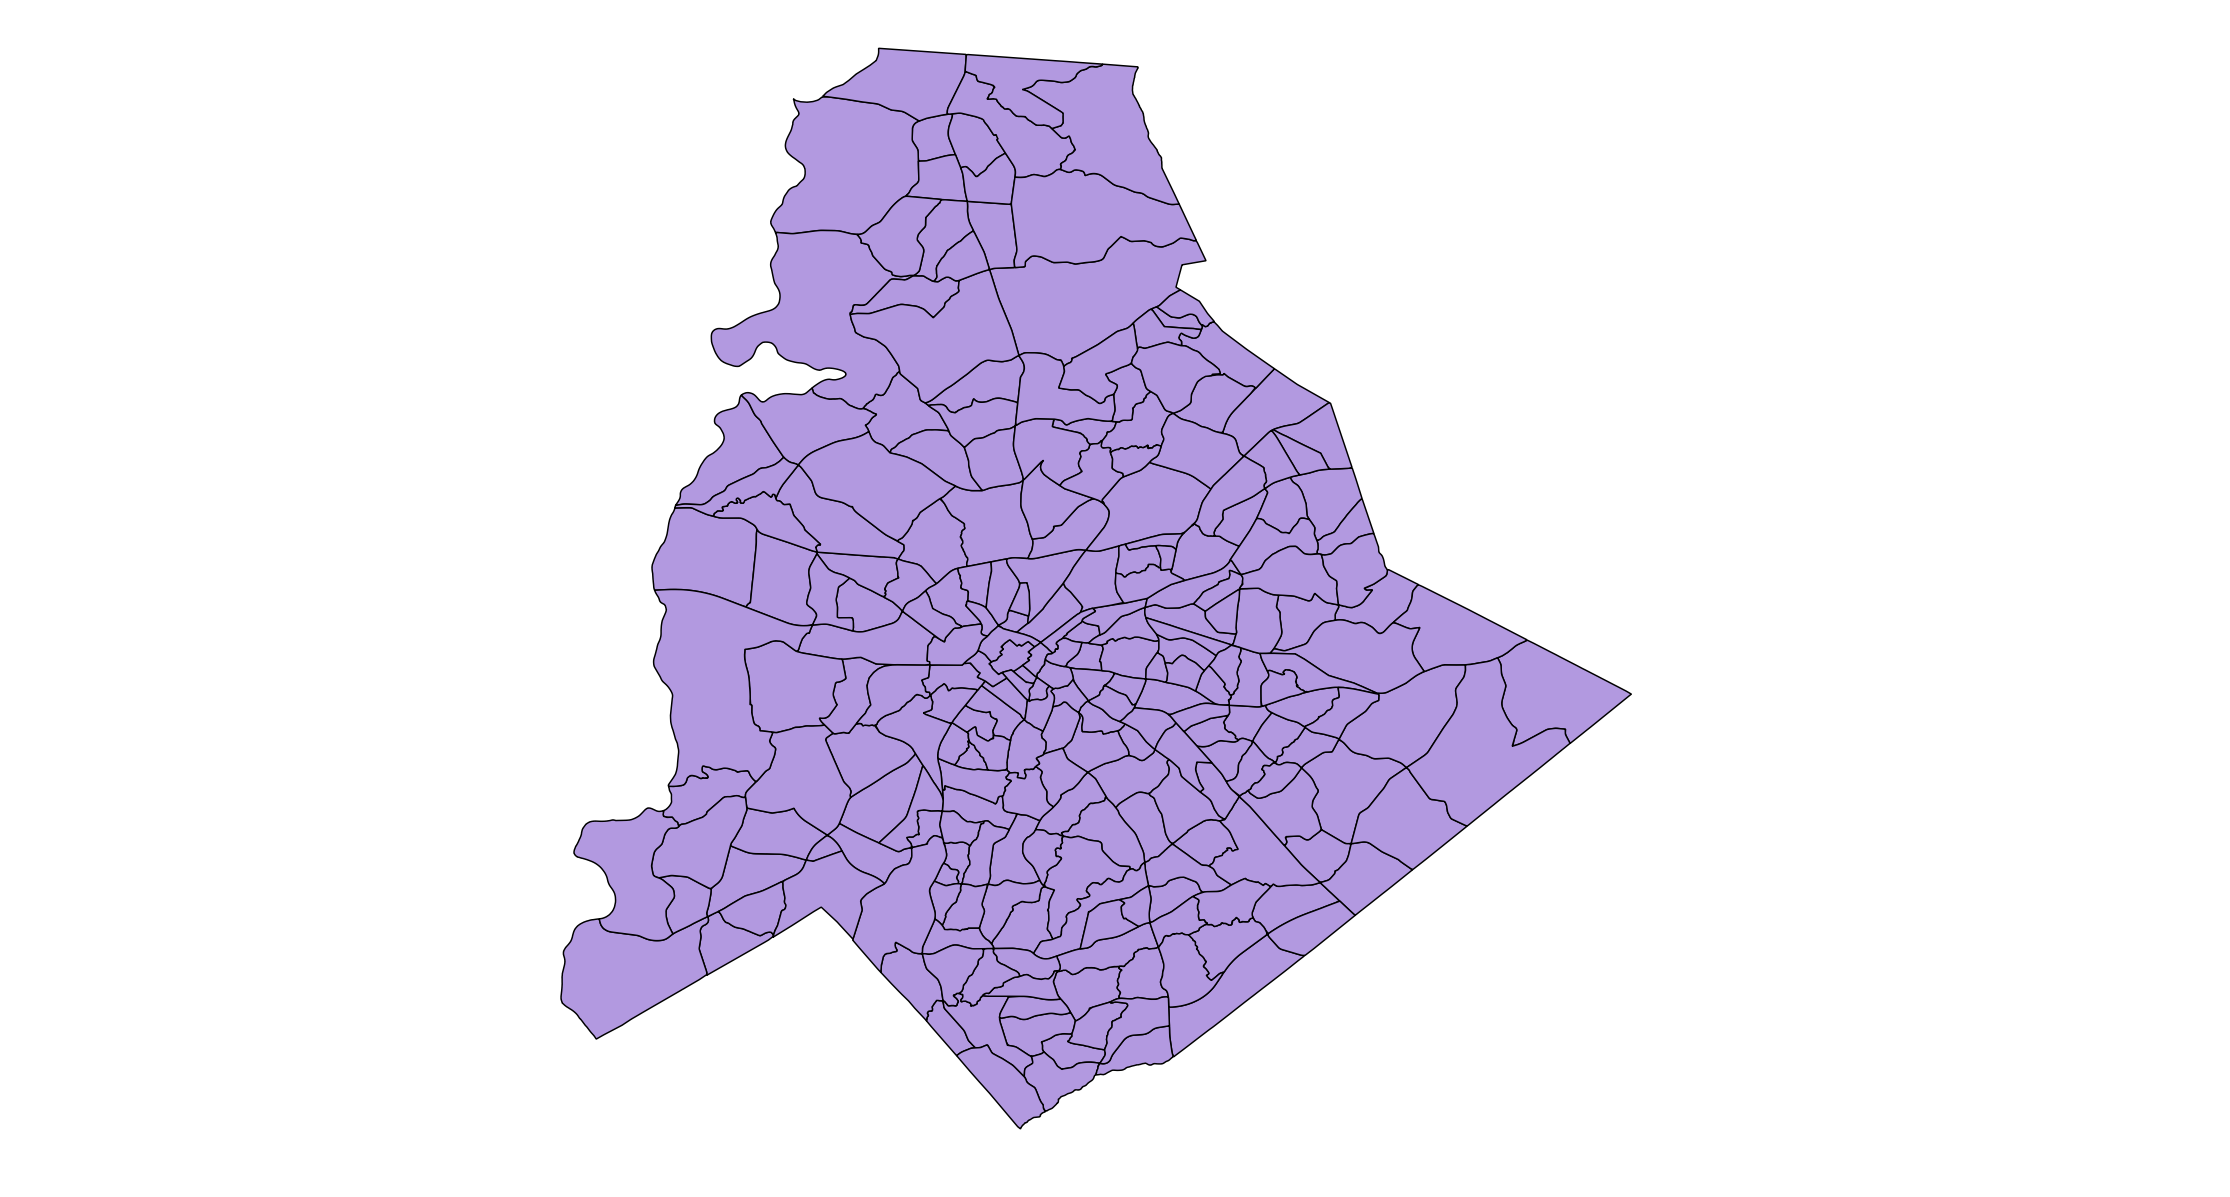
\includegraphics[width=1\linewidth]{Meck.eps}
  \caption{Mecklenburg County tracts}
  \label{fig:meck_tracts}
\end{subfigure}%
\begin{subfigure}{.5\textwidth}
  \centering
  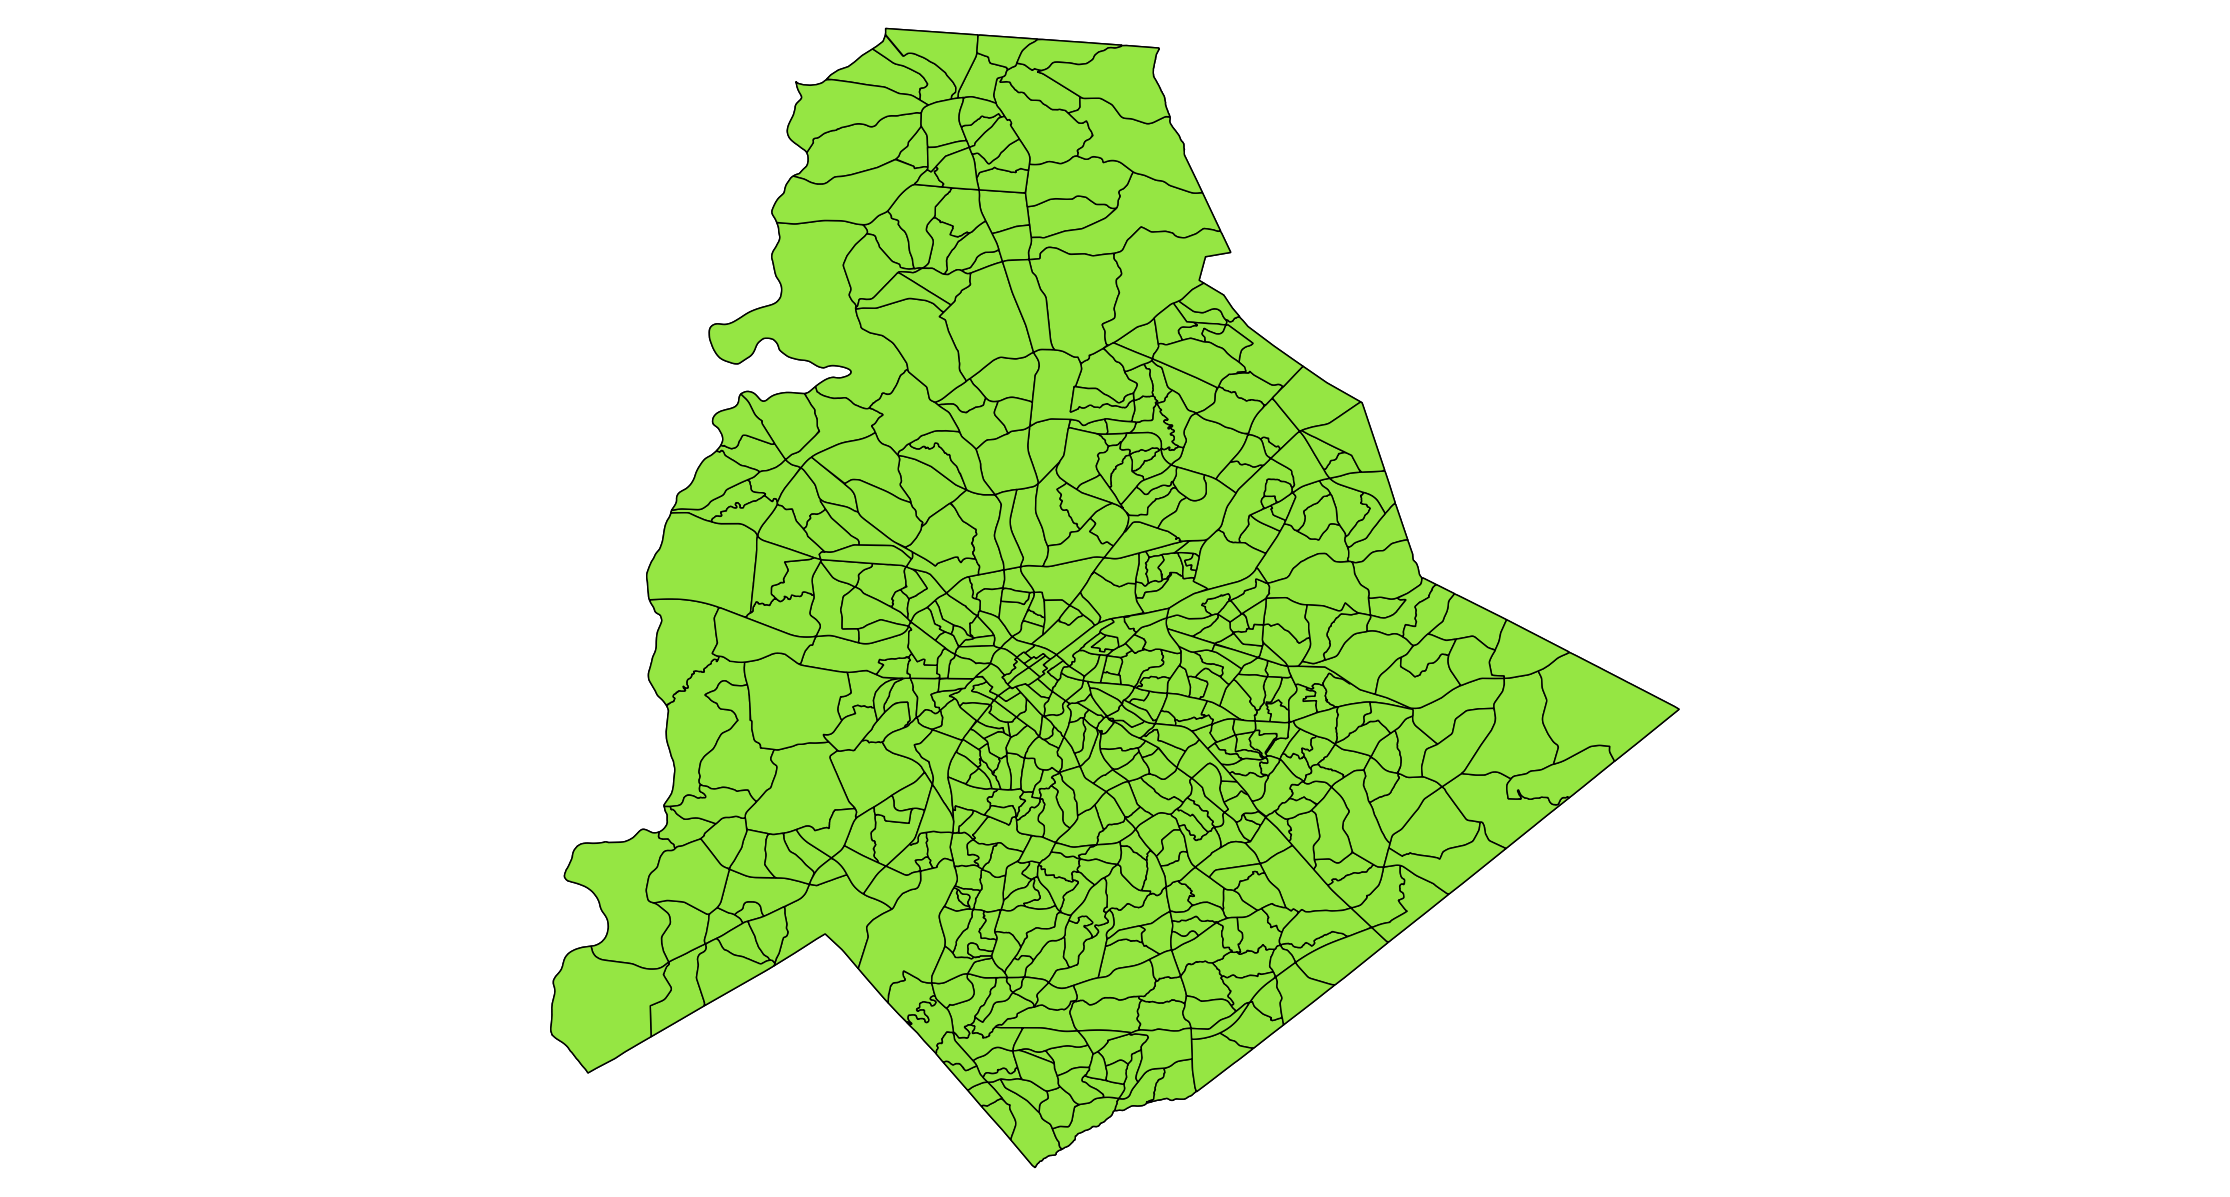
\includegraphics[width=1\linewidth]{meck_bg.eps}
  \caption{Mecklenburg County block groups}
  \label{fig:meck_bg}
\end{subfigure}
\caption{Mecklenburg County divided into tracts (\ref{fig:meck_tracts}) and block groups (\ref{fig:meck_bg})}
\label{fig:bg_tract_cmp}
\end{figure}


\subsection{Week One}
In Week One of Winter Term, I continued to work on the shapefile generation program. The new block group functionality also required several new tests to ensure records were organized correctly within the shapefile. I also worked on documenting the mnemonics used to identify the meaning of values in the shapefile and sent these to Levrum. 

\subsection{Week Two}
I finalized the shapefile generation program in Week two. Finalizing the program involved more work on block group functionality, as well as implementing a command-line interface for obtaining data from any county at both the block group and tract level. Kien and I also restarted our weekly TA meetings with Daniel. Daniel proposed a new format for our meetings, in which we define the requirements we are working on and present something to Daniel each week. 

We also had a meeting with Levrum, in which we debriefed on the shapefile generation program and discussed next steps in the project. Now that we had the target county and its demographics, we would now need to add data on the number and types of incidents that have occurred in each of the tracts or block groups in that county. After the meeting, I spent some time researching Python libraries for counting points in the tracts, which are represented as polygons in the shapefile. I also spent some time researching whether we should migrate our code from Python 2 to Python 3, due to some library compatibility concerns I had, but I ultimately determined that the migration was not necessary at this point.

\subsection{Week Three}
In Week 3, I spent more time researching Python libraries for counting points inside shapefile geometries. I also familiarized myself with the same functionality in QGIS (see Figure \ref{fig:pts_in_meck}) so that I could understand and visualize what my code was accomplishing and compare the results of my algorithm to QGIS's output. I settled on the Geopandas library after discovering that its algorithm for counting points in polygons was running about five times faster during my test cases than the Pyshp, the library I used for the previous shapefile transformation program. I then began implementing code to count incidents in each tract or block group. I added a few unit tests as I coded to ensure I was getting appropriate results during intermediate steps. As of the end of Week 3, I was able to append distinct incident counts to each tract record. Preliminary manual testing, which consisted of comparing random fields to those in QGIS, looked promising at this stage, but I had not yet implemented automated testing.

\begin{figure}[h!]
    \centering
    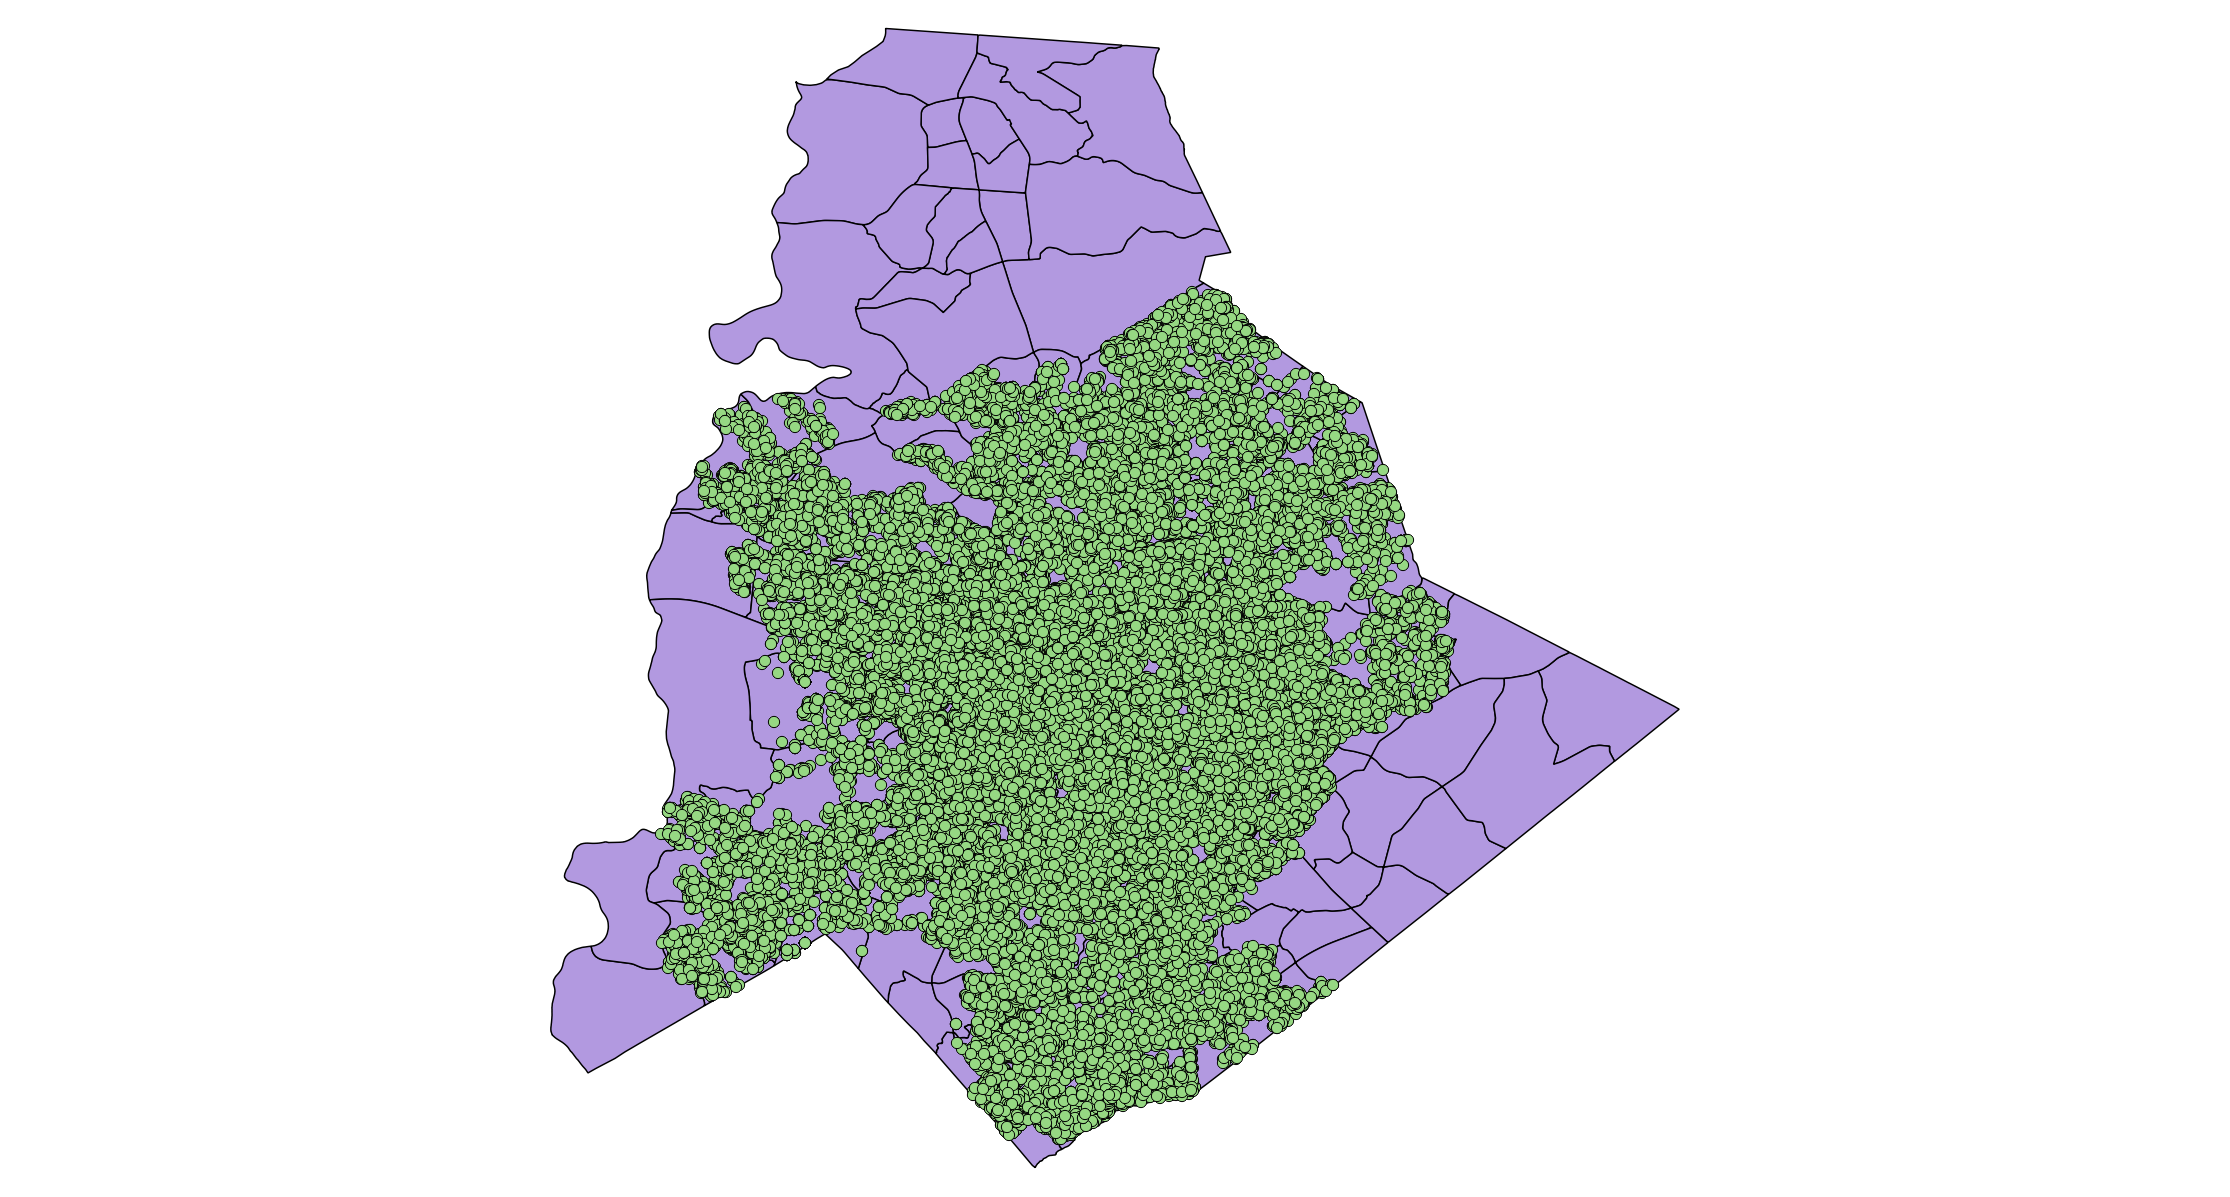
\includegraphics[scale=0.25]{pts_in_meck.eps}
    \caption{Incidents in the response area within Mecklenburg County}
    \label{fig:pts_in_meck}
\end{figure}


\begin{figure}
\centering
\begin{subfigure}{.5\textwidth}
  \centering
  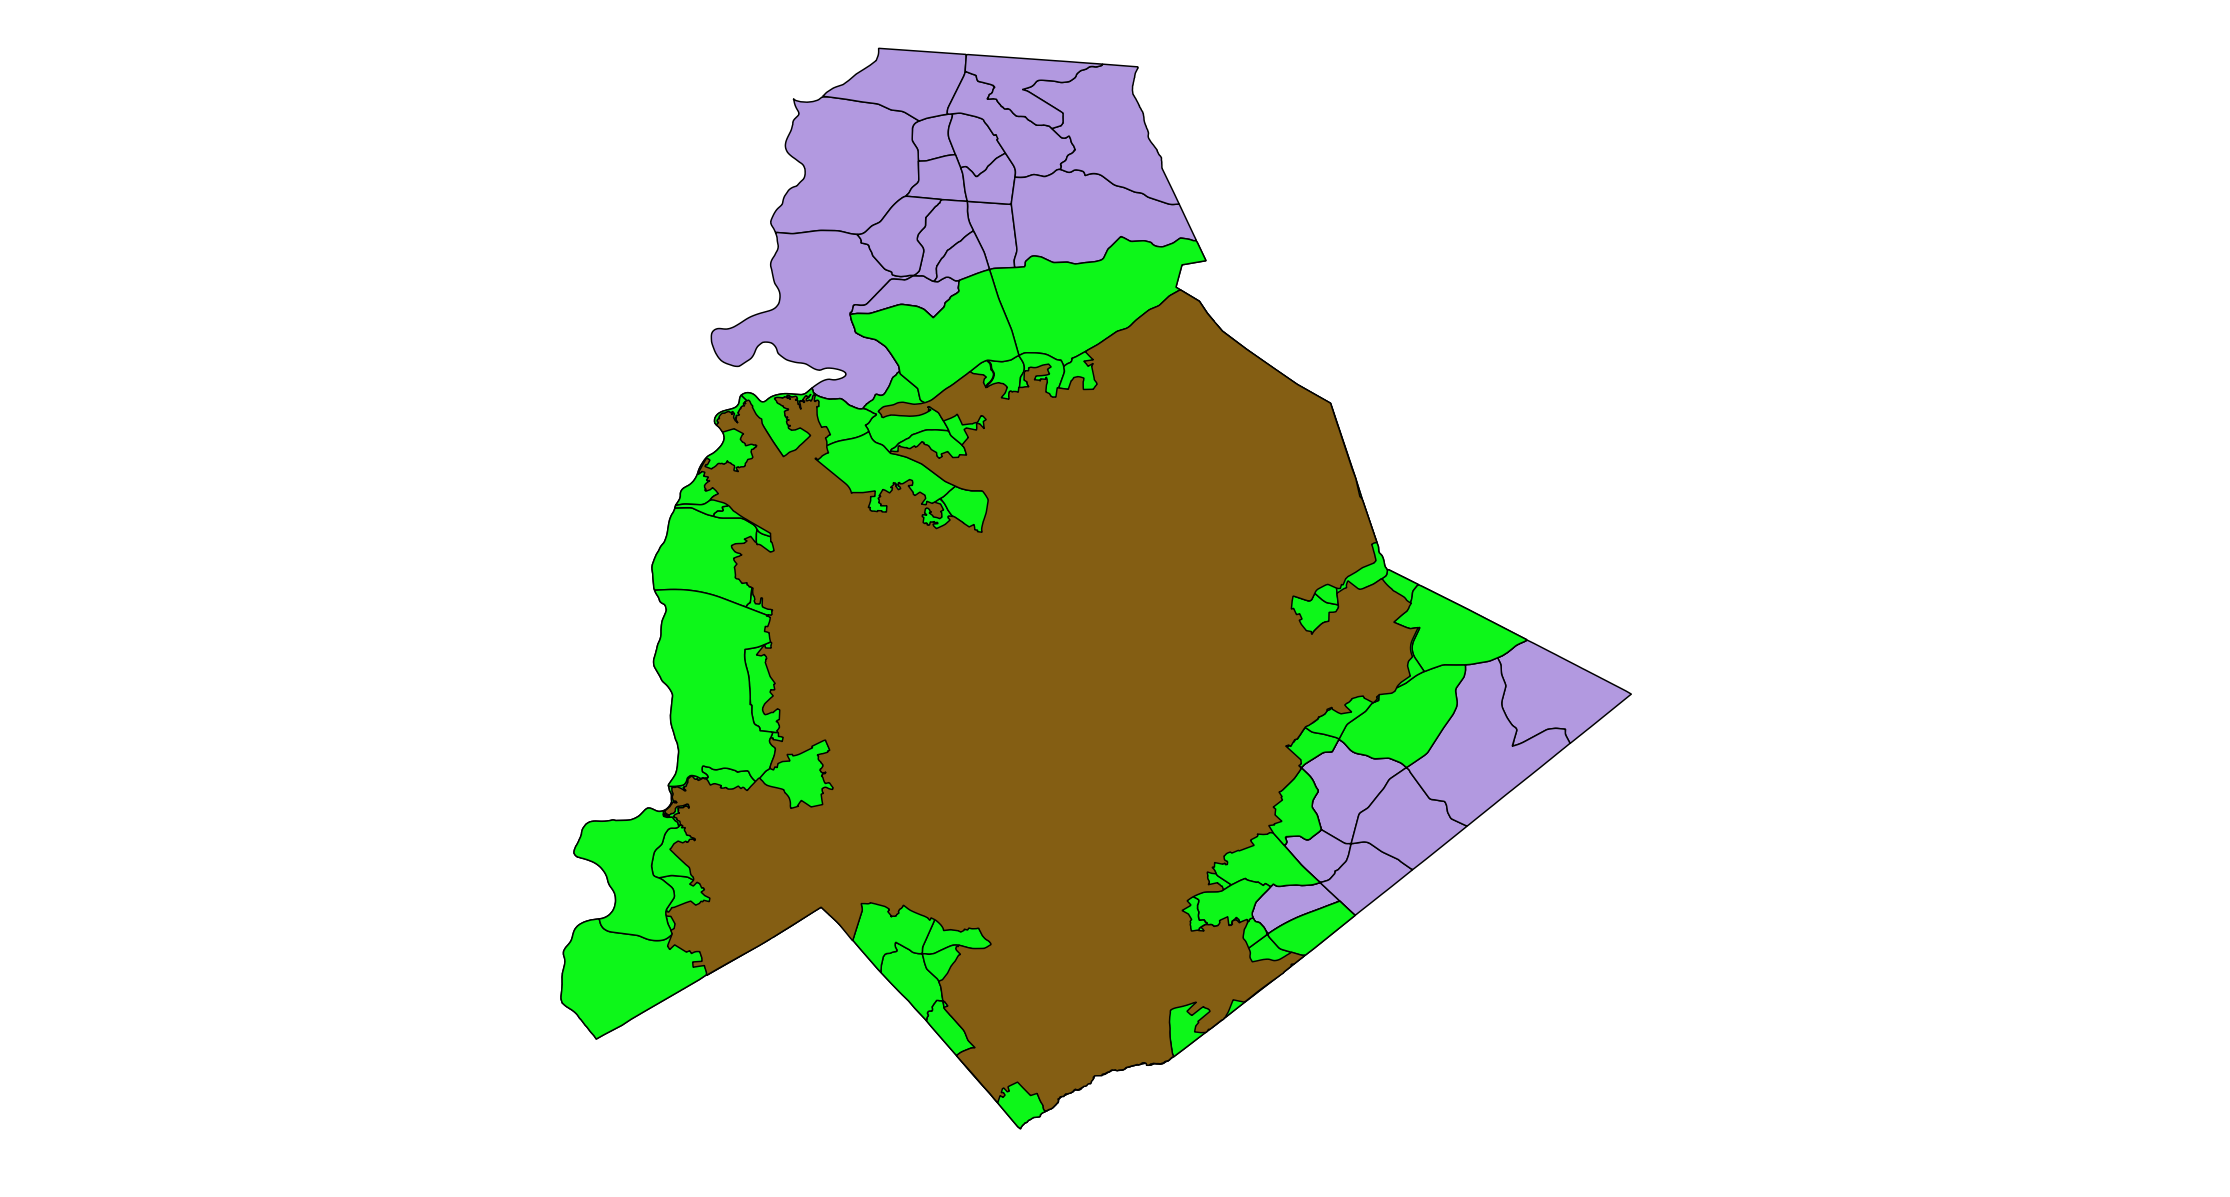
\includegraphics[width=1\linewidth]{Meck_Int_resp.eps}
  \caption{Response area (brown) overlaid on intersection (green) overlaid on Mecklenburg County (purple)}
  \label{fig:meck_int_resp}
\end{subfigure}%
\begin{subfigure}{.5\textwidth}
  \centering
  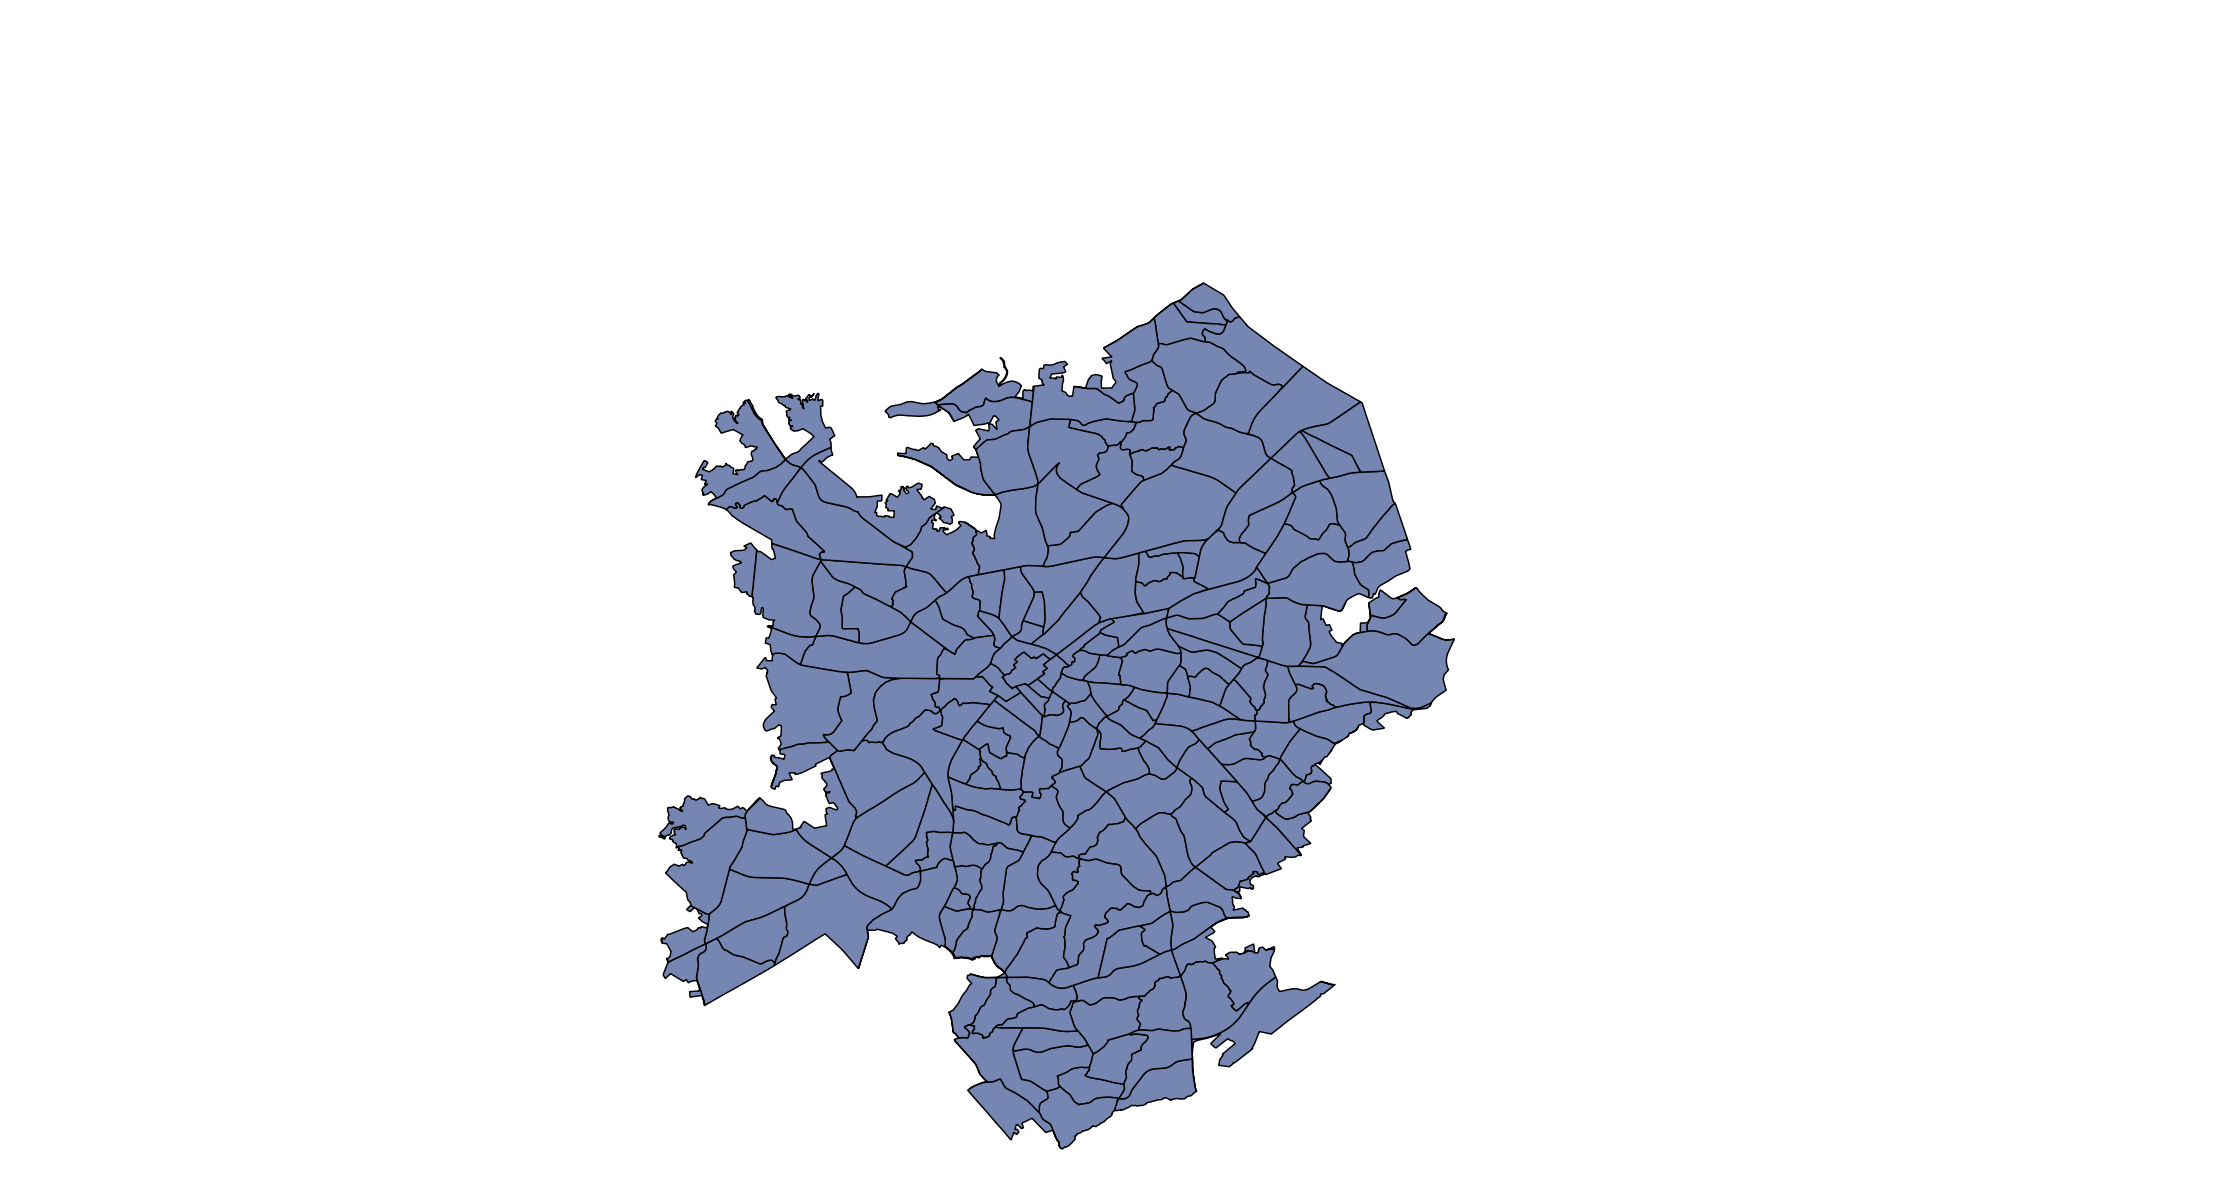
\includegraphics[width=1\linewidth]{clip.eps}
  \caption{Clip of response area against tracts}
  \label{fig:clip}
\end{subfigure}
\caption{Response area intersection (\ref{fig:meck_int_resp}) and clip (\ref{fig:clip}) with Mecklenburg County tracts}
\label{fig:clip_int_cmp}
\end{figure}


\subsection{Week Four}
During Week 4, I continued to work on automated testing for counting incidents in tracts. One of my tests uncovered a bug: the shapes and records in the generated shapefile were not lining up. I spent a considerable amount of time reading and tinkering with the code to see if I could see how the shapes and records correlate. After establishing with certainty that there is a 1:1 mapping between shapes and records in a shapefile, I realized I was reading in the wrong shapefile. As a result of this mistake, I modified the directory structure to more clearly indicate where each type of shapefile is located.

\subsection{Week Five}
I almost completely finished the code to count incidents in each census tract in Week 5. For the majority of the week, I had still not determined why we could not see the attributes of the generated shapefiles in ArcMap, a popular, proprietary geospatial analysis program, but could see them in QGIS. Kien's initial results for a geographically weighted regression (GWR) and other regression methods did not yield good results (see Kien's description in Section \ref{k_regression}). At our meeting with Levrum, we determined that this was likely because the incident response area is smaller than Mecklenburg County. Thus, we have some Census tracts that may have a large population, yet according to our data, no incidents occurred in those tracts.

We agreed Census tracts outside the response area needed to be eliminated. Sean Ermer, an employee at Levrum, sent us a shapefile containing the geography of the response area provided by Levrum's clients. We discussed a few options for eliminating irrelevant geography during the meeting and agreed that finding the intersection of tracts and response area should be sufficient; however after some experimentation, it appeared to me that it would be worth investigating the creation of a clip of the geometry of the response area within the county. A clip would exclude all geography outside the response areas, and it would also require adjustment of some values in the demographics. For example, if only $50\%$ of a tract is in the clip, the population listed for that tract should be cut in half.

Over the remainder of the week and weekend, I created a program to generate both an intersection and a clip of Mecklenburg County against the response area. Both of these files will be used to create new regression analyses in Week 6 and in our machine learning modules later in the term.

\subsection{Summary and Remaining Work}
All of my work up to this point in Winter Term has been on data ingestion because Levrum's primary focus is currently on obtaining data for Mecklenburg County, with which we can run analyses as a proof of concept. I have an unpolished, but relatively well-tested, system that accomplishes the following:

\begin{enumerate}
    \item Generating a shapefile for a target county with demographics for each tract or block group.
    \item Intersecting and clipping that shapefile against a response area shapefile and adjusting values as needed.
    \item Counting incidents that occur within each shape (tract or block group) contained in the clipped or intersected shapefile.
\end{enumerate}

Items two and three above need to be generalized for other response areas and counties, and Levrum and I are currently discussing how we should match up demographics with incident counts, since our Census data is obtained over 5-year periods. I will need to adapt the code to aggregate counts in the way Levrum determines most appropriate and then generalize the code to other use cases.

After that, I have to begin work on feature extraction, which consists of creating tools for transforming data I gathered in my previous work into values that are useful for the machine learning module. As an example of feature extraction, I will be finding the difference between population in one year from the population in the previous year because a dramatic change in population for a given area may affect the number of certain types of emergency calls generated in that area.

I also still have yet to work on an application interface. The interface is less of a priority for Levrum at this point, as they are concerned with attaining a proof of concept for potential clients in Mecklenburg County, NC.

\end{singlespace}

\section{Kien's Progress} \label{kien_weekly_summ}
\begin{singlespace}
% TODO
\subsection{Winter Break} \label{k_winter}

\subsection{Winter Term} \label{k_wterm}

\subsubsection{Week One} \label{k_w1}

\subsubsection{Week Two} \label{k_w2}

\subsubsection{Week Three} \label{k_w3}

\subsubsection{Week Four} \label{k_w4}
% Kien, please label whichever section you start talking about the initial 
% regression results
% with this: 
\label{k_regression}

\subsubsection{Week Five} \label{k_w5}


\end{singlespace}
% REFERENCES
%\newpage    
%\bibliography{WMidtermRepRef}{}
%\bibliographystyle{ieeetr}

\end{document}

